\section{Overview}\label{sec:overview}


%Given a 2D expanded layout of a carton, our system allows users to explore the shape and structure of corresponding models.

%\begin{figure}
%	\centering
%	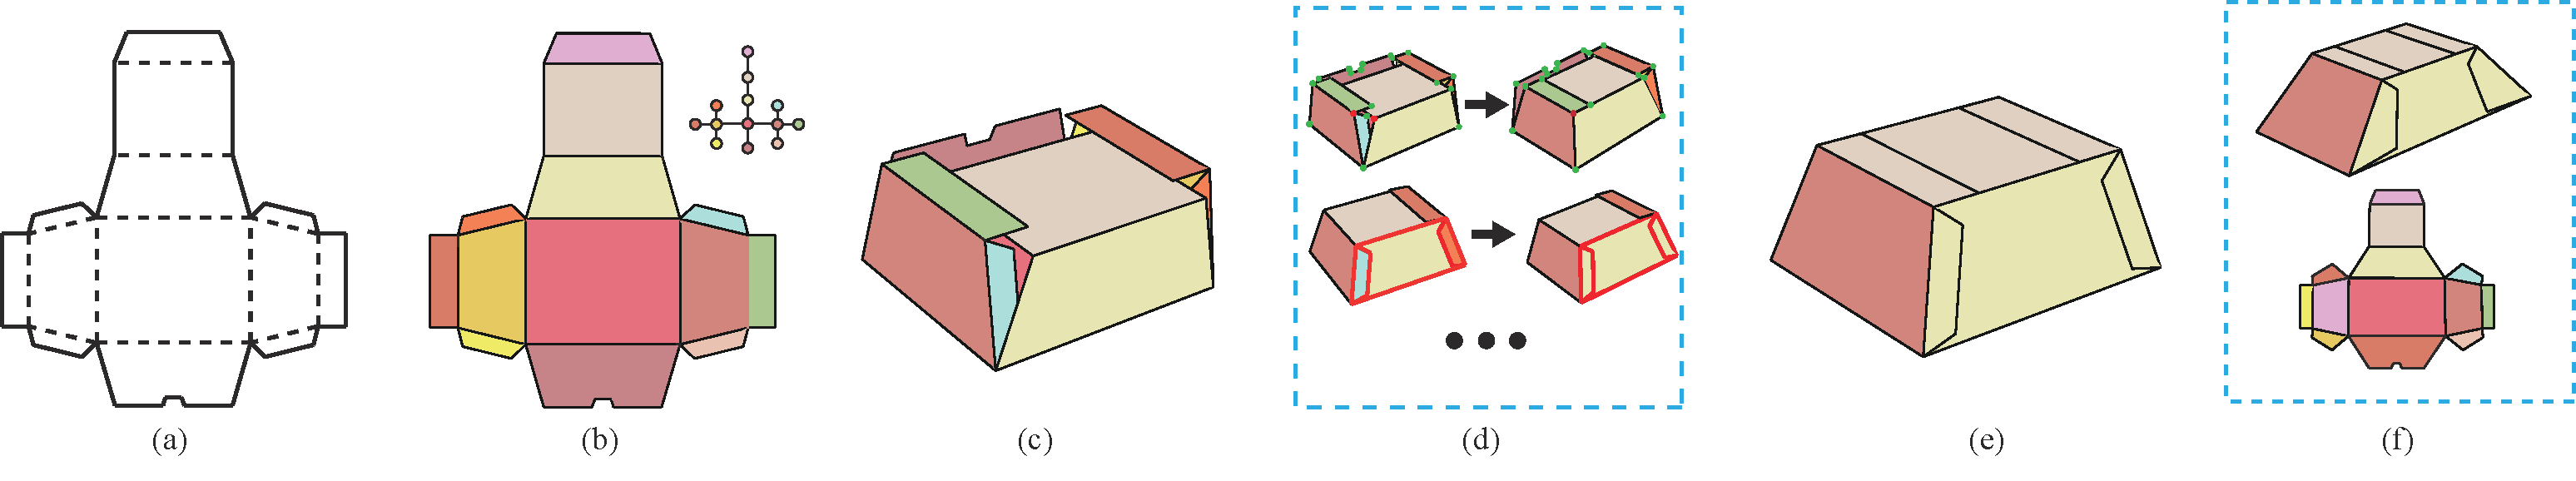
\includegraphics[width=0.9\textwidth]{images/overview}
%	\caption{Given a 2D layout (a), we first extract its 2D mesh (b), with different face in different color. By providing each folding edge with a specific angle, we can construct an initial 3D model (c). The final carton model (e) is built through the shape optimization based on the information acquired from user interactions (d).}
%	\label{fig:overview}
%\end{figure} 

 
Figure~\ref{fig:overview} shows the overview of our algorithm. 
As shown in Figure~\ref{fig:overview}(a), the input 2D design layout of a carton consists of a set of cutting edges (solid lines) and folding edges (dashed lines).
%
Given the 2D layout, an undirected graph is built and faces are extracted by finding minimum cycles in the graph, as Figure~\ref{fig:overview}(b) shows. 
%Each face is filled with a unique color. %by ignoring the holes in the plane
The 2D layout therefore can be represented by a polymesh $\mathcal{L}=(V,E,F)$, where $V$ is the set of vertexes, $E$ is the set of all edges, and $F$ is the set of faces. 
The edge set $E=E_c\cup E_f$, where $E_c$ is the set of cutting edges, and $E_f$ is the set of folding edges.
%
To build a 3D carton model $\mathcal{M}=(V, E, F)$ from the 2D layout $L$, while they share the same topology, we compute the 3D coordinates of all vertexes in $V$. 
%

However, it is not intuitive to analytically define the desired final 3D shape from a 2D layout. 
One possible way is to detect all the possible geometric constraints such as vertex merging, face parallelism, adjacent face orthogonality, and then to integrate all these possible constraints together to form a large equation system. 
But the challenge is that these local constraints can not well describe complicated and creative designs. 
Moreover, there are many ambiguities when detecting these constraints in a 2D layout that consists of many repeated edges and faces. 
%
We propose a two-step algorithm based on the observation that humans usually fold edges with a right angle to get a rough shape and then merge vertexes or edges to get a stable 3D carton.
% Our algorithm consists of two steps. 
First, an initial 3D model (Figure~\ref{fig:overview}(c)) is constructed based on a specific angle along each fold edge, as described in Sec.~\ref{sec:initialization}.
The user can then manipulate and explore 3D shapes of the canton based on a series of suggestive operations provided by our system. 
%
The final model is shown in Figure~\ref{fig:overview}(e).

% is finally built through the optimization based on the information acquired from user interaction. 
%\cxj{Modify this overview when you have new figure.}
%{\color{blue}{Furthermore, our system allows users modify the final 3D model to the desired shape, and automatically enforce the shape constraints reversely to the flat polymesh to get a deformable layout as shown in Figure~\ref{fig:overview} (f).}}


\comments{
  a flat polymesh $L$ is created from a 2D design layout of a box, then we deform the input polymesh into its 3D realization $R_i$ according to the predicted angles along each of its fold edges, and through optimization, generate final model $R_f$. A polymesh consists of a set of vertices, edges and faces $M = (V,E,F)$, the number of vertexes $V$, edges $E$ and faces $F $ vary from one mesh to another. However, a pair of $(L,R_f)$ as the 2D layout and its corresponding 3D realization share the same topology and therefore they have the same number of vertices, edges and faces. A flat mesh as a 2D layout $L$ has its $z$ component of each vertex set to be a constant zero: $X_z(\mathbf{v}) \equiv 0$ where $X = (X_x,X_y,X_z)$ is the vertex coordinate, and its normal of each face set as $(0,0,1)^T$: $\mathbf{n}(f) \equiv (0,0,1)^T$, where $f \in F$.
}



